\documentclass[runningheads]{llncs}
\usepackage[T1]{fontenc}
\usepackage{graphicx}
\usepackage{booktabs}
\usepackage{amsmath,amssymb}
\usepackage{microtype}
\usepackage{url}
\usepackage{cite}

\InputIfFileExists{generated/macros.tex}{}{}
\newcommand{\logit}{\operatorname{logit}}

\pdfinfoomitdate=1
\pdftrailerid{}
\pdfsuppressptexinfo=-1
\begin{document}
\title{Supplementary Material:\\ CARF: Bounded Anchored Fusion for Multimodal Prediction with Unreliable Modalities}
\titlerunning{CARF: Bounded Anchored Fusion (Supplement)}
\author{Anonymous Authors}
\authorrunning{Anonymous Authors}
\institute{Anonymous Institution}
\maketitle

\setcounter{section}{0}
\renewcommand{\thesection}{S\arabic{section}}
\renewcommand{\thetable}{S\arabic{table}}
\renewcommand{\thefigure}{S\arabic{figure}}

\section{Data and preprocessing}

\paragraph{Patient linkage.} Identifiers are matched explicitly across the clinical, expression, and imaging sources of each cohort. Technical expression replicates are averaged after checking that their response labels agree. Only pretreatment variables enter the models; treatment arm, follow-up, and survival variables are excluded. The complete-case analysis contains \NDev{} I-SPY2 patients (\NDevPos{} with pCR) and \NExt{} I-SPY1 patients (\NExtPos{} with pCR).

\paragraph{Expression.} Both cohorts are measured with microarrays (GEO GSE194040 and GSE22226). We intersect gene symbols across the two platforms and, for each patient separately, replace the observed values by their average ranks divided by the number of observed genes. Missing entries remain missing and are imputed by the training-set median inside every expert fit. The variance filter (3{,}000 genes) and the ANOVA selection (250 genes) are refitted inside every inner and outer training partition.

\paragraph{MRI features.} The MRI expert uses \NMriFeat{} features computed inside the supplied tumor mask from the precontrast, early postcontrast, and late postcontrast phases of the pretreatment examination: 54 signal summaries, six shape descriptors (log volume, log surface area, bounding-box extent, sphericity, axis ratio, and log maximum extent), two kinetic fractions, and four texture descriptors computed from masked nearest-neighbour co-occurrences of the enhancement map. Signal is normalized by the patient's positive precontrast median. Input checks cover image and mask shape agreement, finite tumor signal, a minimum mask size, voxel spacing, and mask validity. The features are fixed and do not use outcome labels.

\paragraph{Experts.} All experts are logistic regressions with class-balanced weights: $C=0.1$ for the transcriptomic expert and $C=1$ for the clinical and MRI experts, with training-fitted median imputation and standardization.

\section{Full comparison tables}

Table~\ref{tab:mainfull} reports all fusion baselines and ablations, including offset logistic regression with mask augmentation, an MLP gate on probabilities and availability indicators, and CARF without MRI; Table~\ref{tab:stressfull} adds Gaussian noise on the expert outputs (SD 0.25) and the largest observed displacement from the anchor logit, and Table~\ref{tab:inputfull} reports all input-level corruption levels.

\begin{table}[h]
\centering
\caption{Full version of the main comparison table. AP denotes average precision.}
\label{tab:mainfull}
\small
\InputIfFileExists{generated/tab_main_full.tex}{}{\textit{[table pending]}}
\end{table}

\begin{table}[h]
\centering
\caption{Full version of the stress table, with output-level noise and the largest absolute change from the anchor logit, $\max|z-a|$.}
\label{tab:stressfull}
\small
\InputIfFileExists{generated/tab_stress_full.tex}{}{\textit{[table pending]}}
\end{table}

\begin{table}[h]
\centering
\caption{External AUROC under all input-level corruption levels (mean of 30 realizations). RNA drop: fraction of genes set to missing before rank normalization; RNA shift: fraction of genes shifted and shift size in log-ratio units; MRI noise: Gaussian noise in training standard deviations; MRI drop: fraction of features set to missing.}
\label{tab:inputfull}
\small
\InputIfFileExists{generated/tab_input_full.tex}{}{\textit{[table pending]}}
\end{table}

\section{Independent frozen cohorts: GSE25066 and GSE20194}

We evaluate the external models of the main paper, fitted once on all of I-SPY2 and never refitted, on two public neoadjuvant breast cancer cohorts measured with Affymetrix microarrays. For each cohort, the transcriptomic expert is refitted on I-SPY2 restricted to the genes shared with that cohort (12{,}015 for GSE25066 and 12{,}148 for GSE20194), which uses no labels of the new cohort; all other settings are unchanged, and MRI is absent for all patients. GSE25066 contains 83 I-SPY1 patients, 62 of which belong to our I-SPY1 cohort; we exclude them, which leaves 409 patients (85 with pCR) as our primary independent test. GSE20194 (230 distinct patients, 48 with pCR) is not independent: 186 of its patients are duplicates of GSE25066 arrays.

On GSE25066, both experts transfer poorly (AUROC 0.662 for the clinical and 0.669 for the transcriptomic expert). CARF reaches 0.653, i.e., it adds no discrimination to the clinical expert ($-0.010$, $[-0.023,0.001]$), and it is below the fusion baselines, significantly so for the robust offset model (0.702, $[-0.093,-0.006]$). With a permuted RNA output or half of the genes missing, CARF stays at the clinical level (0.662 in both cases), whereas offset logistic regression drops to 0.602 under permutation ($+0.060$, $[0.025,0.095]$), and stacking (0.639) and the ModDrop MLP (0.645) lose accuracy with half of the genes missing (intervals including zero). The largest displacement of CARF from the anchor is 0.48 logits, as opposed to 1.5--6.0 for the other fusion models. The results on all 488 labeled patients, including I-SPY1, are similar (CARF 0.658, clinical 0.669).

On GSE20194, the clinical expert dominates (0.821 versus 0.716 for the transcriptomic expert), CARF reaches 0.816, and no fusion model improves upon the clinical expert. With half of the genes missing, CARF (0.812) is above stacking ($+0.047$, $[0.023,0.070]$), mask-stacking ($+0.028$, $[0.010,0.045]$), the ModDrop MLP ($+0.035$, $[0.014,0.055]$), and offset logistic regression ($+0.048$, $[0.018,0.077]$), and not distinguishable from the robust offset model.

\section{Third domain: METABRIC}

We also apply CARF to a different clinical task with its own training and test data, fixed before fitting any model. On METABRIC, the outcome is death from breast cancer within five years (patients censored before five years, including other-cause deaths, are excluded); the anchor is a clinical expert on age, tumor size, grade, number of positive lymph nodes, ER status, and HER2 status, and the optional modality is microarray expression, with the same expert and fusion settings as in the main paper. We train on cohorts 1--2 (734 patients, 132 events) and test on cohorts 3--5 (1{,}091 patients, 205 events); the MRI column is absent for all patients.

The clinical expert reaches a test AUROC of 0.739 and the expression expert 0.660, i.e., the anchor dominates, and CARF uses a small effective budget (largest displacement 0.28 logits, as opposed to 2.1--5.0 for the other fusion models). CARF improves upon the clinical expert (0.749; paired interval $[0.002,0.019]$) and is not distinguishable from stacking (0.753; $[-0.015,0.005]$) or the other fusion baselines. When the expression output is permuted, CARF is above stacking ($+0.017$, $[0.013,0.021]$), mask-stacking ($+0.009$, $[0.006,0.011]$), and the ModDrop MLP ($+0.012$, $[0.009,0.015]$), but slightly below the clinical expert ($-0.004$) and the robust offset model ($-0.001$). As in the main paper, the class-balanced models, including CARF, are poorly calibrated to the prevalence of the test cohort (ECE 0.22 for CARF versus 0.04 for the unweighted offset models).

\section{Paired intervals for all stress scenarios}

Table~\ref{tab:stressci} reports paired bootstrap intervals for the difference in external AUROC between CARF and each comparator in every stress scenario of Table~2 in the main paper, computed as for RNA permutation (2{,}000 patient resamples, 30 realizations held fixed). Intervals that exclude zero in favor of CARF occur under RNA permutation for all comparators and with 60\% of the MRI features missing against offset logistic regression; no interval excludes zero in favor of a comparator.

\begin{table}[h]
\centering
\caption{CARF minus comparator external AUROC, median [2.5\%, 97.5\%] over 2{,}000 paired patient resamples, for all stress scenarios.}
\label{tab:stressci}
\InputIfFileExists{generated/tab_stress_ci.tex}{}{\textit{[table pending]}}
\end{table}

\section{Naturally missing modalities}

Table~\ref{tab:natural} reports the full results for the I-SPY1 patients with naturally missing modalities discussed in the main paper.

\begin{table}[h]
\centering
\caption{External AUROC and Brier score on I-SPY1 patients with naturally missing modalities. Models are frozen; absent modalities are passed as masks to CARF and mask-stacking, contribute zero in offset logistic regression with masks, are ignored by the mean of available experts, and are replaced by a probability of $0.5$ in stacking. \emph{All available} combines the complete cases with both partial subgroups; the 16 patients with clinical data only, for which CARF returns the clinical prediction exactly, are not included.}
\label{tab:natural}
\small
\InputIfFileExists{generated/tab_natural.tex}{}{\textit{[table pending]}}
\end{table}

\section{Training-design corruptions}

The CARF objective uses corruption environments in which one optional expert outputs $0.01$ or $0.99$. Table~\ref{tab:design} reports external AUROC for these corruptions, for a neutral output of $0.5$, and for explicit absence. These scenarios are part of the training design of CARF and are therefore not used for the comparisons in the main paper.

\begin{table}[h]
\centering
\caption{External AUROC under the corruptions used in CARF training, a neutral output ($0.5$), and absence of one or both optional modalities.}
\label{tab:design}
\small
\InputIfFileExists{generated/tab_design_stress.tex}{}{\textit{[table pending]}}
\end{table}

\section{Budget and robustness grid}

Table~\ref{tab:sweep} reports the full grid of budgets $B$ and robust weights $\gamma$. In every configuration, the fitted coefficients sum to at least 0.99, so that the total budget is essentially equal to $B$.

\begin{table}[h]
\centering
\caption{CARF refitted on a grid of budgets $B$ and robust weights $\gamma$. Internal AUROC is the mean $\pm$ SD over the 25 outer folds; external AUROC is reported on intact inputs and with a permuted transcriptomic output (mean of 30 realizations); $b_R$ and $b_M$ are the fitted modality budgets of the external model.}
\label{tab:sweep}
\small
\InputIfFileExists{generated/tab_sweep.tex}{}{\textit{[table pending]}}
\end{table}

\section{Calibration}

All class-balanced models overestimate the prevalence of the external cohort. Table~\ref{tab:calib} therefore reports calibration both for the raw models and after Platt scaling of every model on its own inner out-of-fold predictions, as done for CARF in the main paper, together with calibration intercepts and slopes with 95\% patient-bootstrap intervals. With 112 patients and 31 events, ECE estimates are imprecise, and all Platt-scaled models except offset logistic regression (slope 0.98) have calibration slopes above one on the external cohort, i.e., they are underconfident.

\begin{table}[h]
\centering
\caption{External calibration of raw and Platt-scaled models. Intercept: calibration-in-the-large with the slope fixed at one; slope: logistic calibration slope; 95\% bootstrap intervals in brackets.}
\label{tab:calib}
\scriptsize
\InputIfFileExists{generated/tab_calib.tex}{}{\textit{[table pending]}}
\end{table}

\section{Reliability diagram}

\begin{figure}[h]
\centering
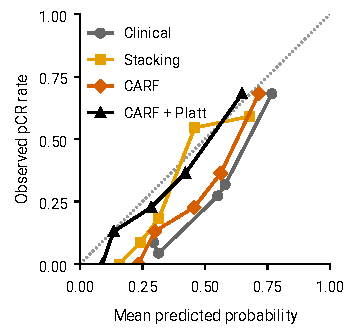
\includegraphics[width=0.6\linewidth]{figures/fig_reliability.pdf}
\caption{External reliability diagram (five equal-count bins) for the clinical expert, stacking, CARF, and CARF with Platt scaling.}
\label{fig:reliability}
\end{figure}

\section{Controlled synthetic study}

The external cohort is small, so we also study CARF on synthetic data with a known generating process. A latent risk $\eta=\beta_Cx_C+\beta_Rx_R+\beta_Mx_M$, with independent standard normal variables, determines $y\sim\mathrm{Bernoulli}(\sigma(\eta+c))$ with a prevalence of about 30\%. Each expert is a logistic regression on a noisy version of its own variable, and all fusion models are fitted on five-fold out-of-fold expert predictions for 1{,}000 training samples and evaluated on 2{,}000 test samples, with 50 replicates per setting. At test time, the strong optional modality $R$ is left intact, replaced by independent noise for a fraction $q$ of samples (silent failure), sign-flipped, removed, shifted by a constant, or made stronger than in training (cost scenario).

Table~\ref{tab:synth} and Fig.~\ref{fig:synth} show a consistent trade-off. On intact data, CARF is below stacking by \SynIntactRange{} AUROC, and in the cost scenario the gap is larger, since the budget prevents CARF from exploiting a modality that has become more informative. When $R$ fails silently for all samples, CARF is above stacking by \SynSilentRange{} AUROC, provided the anchor has an AUROC of at least 0.70; with a weaker anchor, CARF only matches stacking. In this case, however, every fusion model including CARF remains below the anchor alone, as the bounded correction limits but does not remove the damage of an uninformative modality. The same holds when the association of $R$ with the outcome is reversed for all samples: every fusion model falls well below the anchor, and a smaller budget reduces, but does not prevent, the loss (Table~\ref{tab:synth}). Under a constant shift of $R$, which leaves the ranking of an unconstrained linear gate unchanged, CARF loses accuracy, because both the clipping and the nonlinear context functions turn the shift into a change of ranking. Selecting $B$ by inner cross-validation recovers at most 0.01 AUROC on intact data. The synthetic study thus supports the interpretation of CARF as a choice of robustness over clean accuracy, which is favorable only when the anchor is reasonably strong and silent failures of optional modalities are a realistic concern.

\begin{table}[h]
\centering
\caption{Synthetic study: test AUROC (mean over 50 replicates) under failures of the strong optional modality $R$.}
\label{tab:synth}
\small
\InputIfFileExists{generated/tab_synth.tex}{}{\textit{[table pending]}}
\end{table}

\begin{figure}[h]
\centering
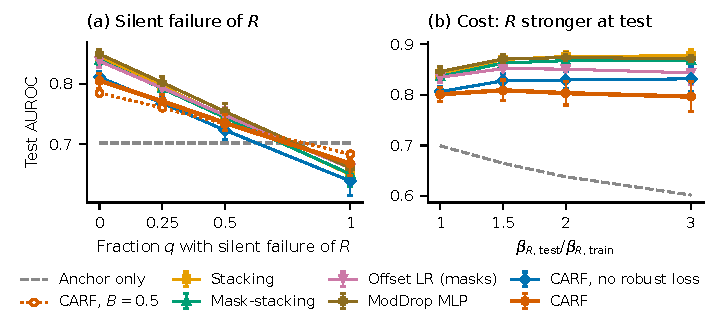
\includegraphics[width=\linewidth]{figures/fig_synthetic.pdf}\\[4pt]
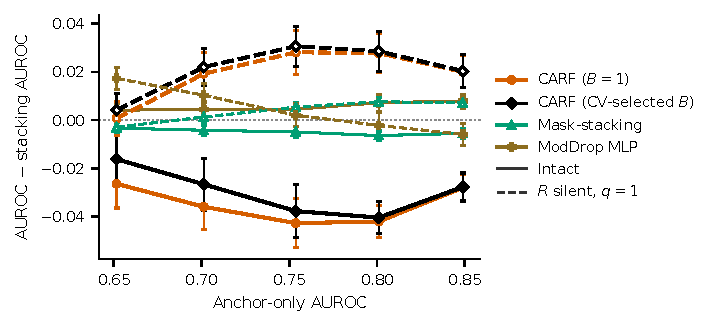
\includegraphics[width=\linewidth]{figures/fig_anchor_sweep.pdf}
\caption{Synthetic study. Top: AUROC under silent failure of $R$ and in the cost scenario. Bottom: AUROC difference to stacking as a function of the anchor AUROC, for intact inputs (solid) and complete silent failure of $R$ (dashed).}
\label{fig:synth}
\end{figure}

\section{Failure of the clinical anchor}

CARF assumes that the anchor is available and correct. To quantify the consequences of violating this assumption, we corrupt the clinical inputs of the external patients before the frozen clinical expert: we flip hormone-receptor or HER2 status for a random 10\% or 25\% of the patients, add Gaussian noise with a standard deviation of 10 years to age, or permute the clinical expert output across patients, each with 30 seeds. Table~\ref{tab:anchor} shows that CARF degrades with its anchor and, when the anchor is severely corrupted, falls below the unconstrained fusion baselines, which can shift weight to the transcriptomic expert.

\begin{table}[h]
\centering
\caption{External AUROC (mean $\pm$ SD over 30 realizations) when the clinical anchor is corrupted.}
\label{tab:anchor}
\small
\InputIfFileExists{generated/tab_anchor.tex}{}{\textit{[table pending]}}
\end{table}

\section{Whole-pipeline permutation test}

To test whether the external performance could arise from a pipeline which learns nothing from the development labels, we permute the I-SPY2 labels, refit all experts and fusion models, and evaluate on I-SPY1 with the true labels. Table~\ref{tab:perm} reports the null distribution over \NPerm{} permutations and the one-sided $p$-value $(1+\#\{\text{null}\ge\text{observed}\})/(1+\NPerm)$.

\begin{table}[h]
\centering
\caption{Whole-pipeline label-permutation test (\NPerm{} permutations).}
\label{tab:perm}
\small
\InputIfFileExists{generated/tab_perm.tex}{}{\textit{[table pending]}}
\end{table}

\section{Second domain: CMU-MOSI}

We apply the same pipeline and fixed settings to binary sentiment prediction (sentiment $\ge0$ versus $<0$) on CMU-MOSI, using the standard training, validation, and test splits and pre-extracted BERT text, COVAREP audio, and FACET visual features, pooled over time by their mean and standard deviation. Each expert is a logistic regression whose regularization is chosen on the validation split; the text expert is the anchor. Gate training uses five-fold out-of-fold expert predictions on the training and validation segments, and all models are evaluated on the \MosiN{} test segments. Stress tests follow the main paper, with 30 seeds for random corruptions.

The text expert reaches a test AUROC of \MosiText{}, while the audio and visual experts reach \MosiAudio{} and \MosiVisual{}. In this regime, the fitted CARF gate is zero for $B\in\{0.5,1\}$ and all ablations, so that CARF returns the anchor exactly, and below $10^{-3}$ for $B=2$. The residuals $d_j=\logit(p_j)-a$ are then almost collinear with $-a$ (correlation 0.98 for audio and 0.997 for visual), so a positive weight would mainly shrink an anchor which is already slightly underconfident (out-of-fold Platt slope 1.09). Table~\ref{tab:mosi} shows that the fusion baselines gain up to \MosiGap{} AUROC on intact data, while CARF has the best worst case over all corruption scenarios.

\begin{table}[h]
\centering
\caption{CMU-MOSI test results. Permuted: expert output permuted across segments (mean of 30 realizations). Worst case: lowest mean AUROC over the \MosiNScen{} corruption scenarios.}
\label{tab:mosi}
\small
\InputIfFileExists{generated/tab_mosi.tex}{}{\textit{[table pending]}}
\end{table}

\paragraph{CMU-MOSEI.} We repeat the same protocol on the larger CMU-MOSEI benchmark (standard splits, 4{,}659 test segments). The pattern is the same as on CMU-MOSI: the text expert reaches a test AUROC of 0.884 and the audio and visual experts 0.644 and 0.636, the fitted gate is exactly zero for $B\in\{0.5,1,2\}$ and all ablations, and CARF therefore coincides with the text expert. The learned fusion baselines are higher by 0.001--0.003 AUROC (stacking 0.887, ModDrop MLP 0.886), a small difference whose paired intervals exclude zero, whereas the worst case of CARF over all corruption scenarios (0.884) is above that of every baseline (0.804--0.882). On the 60 test segments with a naturally missing visual input, the differences between models are not significant.

\end{document}
